\documentclass[12pt]{article}
\usepackage{sbc-template}
\usepackage[utf8]{inputenc}
\usepackage[T1]{fontenc}
\usepackage[english,brazil]{babel}
\usepackage{graphicx}
\usepackage{booktabs}
\usepackage{amsmath,amssymb,amsfonts}
\usepackage{multirow}
\usepackage{array}
\usepackage{float}
\usepackage{caption}
\usepackage{xcolor}
\usepackage{url}
\usepackage[hidelinks]{hyperref}

\graphicspath{{./figures/}}

% Todos os números de resultados vêm de sw/results/*.json via sw/make_paper_assets.py
\newcommand{\VerTests}{14}
\newcommand{\VerTotal}{9.384}
\newcommand{\VerMism}{0}
\newcommand{\SqnrLegacy}{37{,}0}
\newcommand{\SqnrProposed}{99{,}0}
\newcommand{\SqnrMult}{99{,}3}
\newcommand{\ImpLegacyTwelve}{54{,}6}
\newcommand{\ImpLegacyEight}{3{,}43}
\newcommand{\TauErrCpot}{20{,}5\%}
\newcommand{\TauErrCpotTwo}{2{,}4\%}
\newcommand{\TauErrPot}{92{,}5\%}
\newcommand{\LevelsCpot}{8}
\newcommand{\DspCpot}{27}
\newcommand{\DspMult}{54}
\newcommand{\LutCpot}{3.101}
\newcommand{\LutMult}{2.483}
\newcommand{\LutDec}{38}
\newcommand{\MtenkIntA}{128}
\newcommand{\LutIntA}{210}
\newcommand{\MulIntA}{16}
\newcommand{\MtenkTwoA}{32}
\newcommand{\LutTwoA}{370}
\newcommand{\MulTwoA}{0}
\newcommand{\MtenkRthreeA}{26}
\newcommand{\LutRthreeA}{1.019}
\newcommand{\MulRthreeA}{0}
\newcommand{\MtenkIntC}{103}
\newcommand{\LutIntC}{893}
\newcommand{\MulIntC}{64}
\newcommand{\MtenkTwoC}{26}
\newcommand{\LutTwoC}{1.533}
\newcommand{\MulTwoC}{0}
\newcommand{\MtenkRthreeC}{26}
\newcommand{\LutRthreeC}{4.101}
\newcommand{\MulRthreeC}{0}

\newcommand{\YosysVersion}{Yosys 0.33}
\newcommand{\EngK}{256}
\newcommand{\EngM}{512}

\newcommand{\NParams}{68.253}
\newcommand{\SeedsEcg}{5}
\newcommand{\EpochsEcg}{40}
\newcommand{\TrainEcg}{500}
\newcommand{\TestEcg}{4.500}
\newcommand{\SeedsCueA}{5}
\newcommand{\EpochsCueA}{20}
\newcommand{\TrainCueA}{4.000}
\newcommand{\TestCueA}{1.000}
\newcommand{\SeedsCueB}{3}
\newcommand{\EpochsCueB}{20}
\newcommand{\TrainCueB}{2.000}
\newcommand{\TestCueB}{500}
\newcommand{\SeedsWin}{5}
\newcommand{\EpochsWin}{20}
\newcommand{\TrainWin}{4.000}
\newcommand{\TestWin}{1.000}
\providecommand{\acc}[2]{\csname acc@#1@#2\endcsname}
\providecommand{\solved}[2]{\csname solved@#1@#2\endcsname}
\expandafter\def\csname acc@ecg@S0\endcsname{92{,}7}
\expandafter\def\csname solved@ecg@S0\endcsname{5/5}
\expandafter\def\csname acc@ecg@S1\endcsname{92{,}7}
\expandafter\def\csname solved@ecg@S1\endcsname{5/5}
\expandafter\def\csname acc@ecg@S2\endcsname{92{,}8}
\expandafter\def\csname solved@ecg@S2\endcsname{5/5}
\expandafter\def\csname acc@ecg@S2multq15\endcsname{92{,}8}
\expandafter\def\csname solved@ecg@S2multq15\endcsname{5/5}
\expandafter\def\csname acc@ecg@S3\endcsname{91{,}2}
\expandafter\def\csname solved@ecg@S3\endcsname{5/5}
\expandafter\def\csname acc@ecg@S4\endcsname{92{,}4}
\expandafter\def\csname solved@ecg@S4\endcsname{5/5}
\expandafter\def\csname acc@ecg@S5\endcsname{92{,}7}
\expandafter\def\csname solved@ecg@S5\endcsname{5/5}
\expandafter\def\csname acc@ecg@S5cpots32\endcsname{92{,}7}
\expandafter\def\csname solved@ecg@S5cpots32\endcsname{5/5}
\expandafter\def\csname acc@ecg@S5cpots16\endcsname{92{,}6}
\expandafter\def\csname solved@ecg@S5cpots16\endcsname{5/5}
\expandafter\def\csname acc@ecg@S6\endcsname{92{,}6}
\expandafter\def\csname solved@ecg@S6\endcsname{5/5}
\expandafter\def\csname acc@cueA@S0\endcsname{100{,}0}
\expandafter\def\csname solved@cueA@S0\endcsname{5/5}
\expandafter\def\csname acc@cueA@S1\endcsname{100{,}0}
\expandafter\def\csname solved@cueA@S1\endcsname{5/5}
\expandafter\def\csname acc@cueA@S2\endcsname{100{,}0}
\expandafter\def\csname solved@cueA@S2\endcsname{5/5}
\expandafter\def\csname acc@cueA@S2multq15\endcsname{100{,}0}
\expandafter\def\csname solved@cueA@S2multq15\endcsname{5/5}
\expandafter\def\csname acc@cueA@S3\endcsname{25{,}1}
\expandafter\def\csname solved@cueA@S3\endcsname{0/5}
\expandafter\def\csname acc@cueA@S4\endcsname{100{,}0}
\expandafter\def\csname solved@cueA@S4\endcsname{5/5}
\expandafter\def\csname acc@cueA@S5\endcsname{100{,}0}
\expandafter\def\csname solved@cueA@S5\endcsname{5/5}
\expandafter\def\csname acc@cueA@S5cpots32\endcsname{100{,}0}
\expandafter\def\csname solved@cueA@S5cpots32\endcsname{5/5}
\expandafter\def\csname acc@cueA@S5cpots16\endcsname{92{,}4}
\expandafter\def\csname solved@cueA@S5cpots16\endcsname{4/5}
\expandafter\def\csname acc@cueA@S6\endcsname{100{,}0}
\expandafter\def\csname solved@cueA@S6\endcsname{5/5}
\expandafter\def\csname acc@cueB@S0\endcsname{92{,}6}
\expandafter\def\csname solved@cueB@S0\endcsname{9/10}
\expandafter\def\csname acc@cueB@S1\endcsname{92{,}7}
\expandafter\def\csname solved@cueB@S1\endcsname{9/10}
\expandafter\def\csname acc@cueB@S2\endcsname{82{,}2}
\expandafter\def\csname solved@cueB@S2\endcsname{7/10}
\expandafter\def\csname acc@cueB@S2multq15\endcsname{82{,}2}
\expandafter\def\csname solved@cueB@S2multq15\endcsname{7/10}
\expandafter\def\csname acc@cueB@S3\endcsname{24{,}2}
\expandafter\def\csname solved@cueB@S3\endcsname{0/3}
\expandafter\def\csname acc@cueB@S4\endcsname{100{,}0}
\expandafter\def\csname solved@cueB@S4\endcsname{10/10}
\expandafter\def\csname acc@cueB@S5\endcsname{77{,}5}
\expandafter\def\csname solved@cueB@S5\endcsname{7/10}
\expandafter\def\csname acc@cueB@S5cpots32\endcsname{77{,}5}
\expandafter\def\csname solved@cueB@S5cpots32\endcsname{7/10}
\expandafter\def\csname acc@cueB@S5cpots16\endcsname{45{,}4}
\expandafter\def\csname solved@cueB@S5cpots16\endcsname{0/10}
\expandafter\def\csname acc@cueB@S6\endcsname{100{,}0}
\expandafter\def\csname solved@cueB@S6\endcsname{3/3}
\expandafter\def\csname acc@win@S0\endcsname{91{,}7}
\expandafter\def\csname solved@win@S0\endcsname{5/5}
\expandafter\def\csname acc@win@S1\endcsname{91{,}8}
\expandafter\def\csname solved@win@S1\endcsname{5/5}
\expandafter\def\csname acc@win@S2\endcsname{90{,}4}
\expandafter\def\csname solved@win@S2\endcsname{6/10}
\expandafter\def\csname acc@win@S2multq15\endcsname{90{,}5}
\expandafter\def\csname solved@win@S2multq15\endcsname{6/10}
\expandafter\def\csname acc@win@S3\endcsname{60{,}6}
\expandafter\def\csname solved@win@S3\endcsname{0/5}
\expandafter\def\csname acc@win@S4\endcsname{83{,}0}
\expandafter\def\csname solved@win@S4\endcsname{0/10}
\expandafter\def\csname acc@win@S5\endcsname{89{,}9}
\expandafter\def\csname solved@win@S5\endcsname{7/10}
\expandafter\def\csname acc@win@S5cpots32\endcsname{89{,}9}
\expandafter\def\csname solved@win@S5cpots32\endcsname{7/10}
\expandafter\def\csname acc@win@S5cpots16\endcsname{83{,}4}
\expandafter\def\csname solved@win@S5cpots16\endcsname{0/10}
\expandafter\def\csname acc@win@S6\endcsname{90{,}2}
\expandafter\def\csname solved@win@S6\endcsname{4/5}


\title{BitMamba-CV: Co-Projeto Hardware-Algoritmo de Modelos Mamba-2 Tern\'{a}rios com Discretiza\c{c}\~{a}o CPoT para FPGA de Borda}

% TODO: completar afiliação e e-mail institucional
\author{Andr\'{e} Goveia\inst{1}}

\address{Programa de P\'{o}s-Gradua\c{c}\~{a}o -- Aplica\c{c}\~{o}es de Alto Desempenho\\
  \email{andre@instituicao.edu.br}
}

\begin{document}
\sloppy

\maketitle

\begin{abstract}
State space models (Mamba-2) keep a constant-size recurrent state, which makes them attractive for low-cost FPGAs, but their decay factor $\bar{A}_t$ lives close to $1$ and is fragile under shift-only arithmetic. We present \textbf{BitMamba-CV}, a co-design of 1.58-bit ternary Mamba-2 and a multiplier-free selective-scan datapath for the Intel Cyclone~V. We (i) train ternary projections in the Hadamard domain (\texttt{H-BitLinear}) together with an integer-compatible scan (static power-of-two scales, power-of-two $\Delta_t$); (ii) propose the \emph{Complementary Power-of-Two} (CPoT, $\{2^{-k}, 1-2^{-k}\}$) discretisation of $\bar{A}_t$, implemented with one shift and one subtraction; and (iii) show that CPoT is only correct with enough state precision: a 16-bit truncating state freezes long-memory channels (integer datapath SQNR \SqnrLegacy~dB), while a 32-bit state with 10 guard bits and rounding reaches \SqnrProposed~dB, matching a Q1.15 multiplier (\SqnrMult~dB) with fewer DSP blocks; on a delayed-recall task ($L=256$) the same trained model drops from \acc{cueA}{A7cpots32}\% to \acc{cueA}{A7cpots16}\% with the 16-bit state. Ternary models with the integer scan keep FP32 accuracy on ECG5000 and on recall with $L=256$, but ternary training does not converge for most seeds at $L=1024$. All RTL modules are verified bit-exactly against an integer golden model (\VerTotal{} vectors, \VerMism{} mismatches) and characterised with open-source synthesis for Cyclone~V. Timing closure, on-board latency and power are left to the hardware phase and are not claimed here.
\end{abstract}

\begin{resumo}
Modelos de espa\c{c}o de estados (Mamba-2) mant\^{e}m um estado recorrente de tamanho constante, o que os torna atrativos para FPGAs de baixo custo, mas o fator de decaimento $\bar{A}_t$ opera pr\'{o}ximo de $1$ e \'{e} fr\'{a}gil sob aritm\'{e}tica apenas com deslocamentos. Apresentamos o \textbf{BitMamba-CV}, um co-projeto de Mamba-2 tern\'{a}rio (1,58 bit) e de um \emph{datapath} de \emph{scan} seletivo sem multiplicador no decaimento para a Intel Cyclone~V. N\'{o}s (i) treinamos proje\c{c}\~{o}es tern\'{a}rias no dom\'{\i}nio de Hadamard (\texttt{H-BitLinear}) junto com um \emph{scan} compat\'{\i}vel com aritm\'{e}tica inteira (escalas est\'{a}ticas em pot\^{e}ncia de dois e $\Delta_t$ em pot\^{e}ncia de dois); (ii) propomos a discretiza\c{c}\~{a}o \emph{Complementary Power-of-Two} (CPoT, $\{2^{-k}, 1-2^{-k}\}$) de $\bar{A}_t$, implementada com um deslocamento e uma subtra\c{c}\~{a}o; e (iii) mostramos que o CPoT s\'{o} \'{e} correto com precis\~{a}o de estado suficiente: um estado de 16 bits com truncamento congela os canais de mem\'{o}ria longa (SQNR do \emph{datapath} inteiro de \SqnrLegacy~dB), enquanto um estado de 32 bits com 10 bits de guarda e arredondamento atinge \SqnrProposed~dB, equivalente a um multiplicador Q1.15 (\SqnrMult~dB) com menos blocos DSP; numa tarefa de recorda\c{c}\~{a}o com $L=256$, o mesmo modelo treinado cai de \acc{cueA}{A7cpots32}\% para \acc{cueA}{A7cpots16}\% com o estado de 16 bits. Modelos tern\'{a}rios com \emph{scan} inteiro mant\^{e}m a acur\'{a}cia FP32 no ECG5000 e na recorda\c{c}\~{a}o com $L=256$, mas o treinamento tern\'{a}rio n\~{a}o converge na maioria das sementes com $L=1024$. Todos os m\'{o}dulos RTL foram verificados bit a bit contra um modelo de refer\^{e}ncia inteiro (\VerTotal{} vetores, \VerMism{} diverg\^{e}ncias) e caracterizados com s\'{\i}ntese de c\'{o}digo aberto para Cyclone~V. Fechamento de \emph{timing}, lat\^{e}ncia em placa e pot\^{e}ncia ficam para a fase de hardware e n\~{a}o s\~{a}o reivindicados aqui.
\end{resumo}

% =============================================================================
\section{Introdu\c{c}\~{a}o}
% =============================================================================

A infer\^{e}ncia de modelos de sequ\^{e}ncia em FPGAs de baixo custo, como a fam\'{\i}lia Intel Cyclone~V (28\,nm, sem HBM), \'{e} limitada por mem\'{o}ria \emph{on-chip} e por blocos DSP escassos \cite{intel_cyclone5_handbook}. Em Transformers, o \emph{KV-cache} cresce linearmente com o comprimento $L$ da sequ\^{e}ncia; para um modelo de 4 camadas com $D=128$ e chaves/valores em INT8, s\~{a}o $2 \cdot 4 \cdot 128 \cdot L$ bytes, isto \'{e}, 1\,KiB por token. Modelos de espa\c{c}o de estados seletivos (Mamba-1 \cite{gu2024mamba} e Mamba-2 \cite{dao2024transformers}) substituem a aten\c{c}\~{a}o por uma recorr\^{e}ncia linear cujo estado tem tamanho constante em $L$, o que elimina esse crescimento.

Dois obst\'{a}culos aparecem ao mapear o Mamba-2 em uma FPGA de borda. Primeiro, as proje\c{c}\~{o}es lineares (\texttt{in\_proj} e \texttt{out\_proj}) concentram a maior parte dos par\^{a}metros (\ProjRatio{} no modelo usado aqui) e, em INT8, consomem DSPs. Segundo, o decaimento $\bar{A}_t = \exp(-\Delta_t A_h)$ dos canais de mem\'{o}ria longa fica em $[0{,}90;\,0{,}999]$, onde quantiza\c{c}\~{o}es grosseiras alteram a constante de tempo do estado.

Aceleradores Mamba em FPGA j\'{a} usam quantiza\c{c}\~{a}o de 4 e 8 bits em FPGAs de grande porte; o \emph{LightMamba}, por exemplo, usa rota\c{c}\~{a}o e restringe os fatores de \emph{re-escala} da quantiza\c{c}\~{a}o do SSM a pot\^{e}ncias de dois \cite{wei2025lightmamba,fastmamba2025}. Aceleradores tern\'{a}rios (1,58 bit) em FPGA, como \emph{TerEffic} e \emph{TeLLMe} \cite{yin2025tereffic,qiao2025tellme}, visam Transformers. Trabalhos algor\'{\i}tmicos mostram que o Mamba tern\'{a}rio funciona em GPU \cite{yu2025slendermamba,ganesaraja2026ternarymamba,tang2024bimamba}, mas mant\^{e}m o SSM em ponto flutuante.

\textbf{Contribui\c{c}\~{o}es.} (1) Um modelo Mamba-2 com proje\c{c}\~{o}es tern\'{a}rias \texttt{H-BitLinear} \cite{wang2025bitnetv2} e um \emph{scan} treinado j\'{a} com as restri\c{c}\~{o}es do hardware inteiro: escalas est\'{a}ticas em pot\^{e}ncia de dois para $x_t$, $B_t$, $C_t$ e passo $\Delta_t = 2^{-j}$. (2) A discretiza\c{c}\~{a}o CPoT de $\bar{A}_t$, que usa um deslocamento e uma subtra\c{c}\~{a}o, comparada com PoT simples e com um multiplicador Q1.15. (3) Uma an\'{a}lise da precis\~{a}o do estado inteiro, mostrando que a implementa\c{c}\~{a}o ing\^{e}nua (16 bits, truncamento) congela a mem\'{o}ria longa, e a corre\c{c}\~{a}o com bits de guarda e arredondamento. (4) RTL parametriz\'{a}vel (motor matriz-vetor INT8, tern\'{a}rio 2-bit e Radix-3; FWHT; \emph{lane} de \emph{scan}) verificado bit a bit e caracterizado em recursos para Cyclone~V.

\textbf{Escopo.} Este artigo n\~{a}o reporta frequ\^{e}ncia m\'{a}xima, lat\^{e}ncia em placa nem pot\^{e}ncia: esses dados dependem da s\'{\i}ntese no Intel Quartus e da execu\c{c}\~{a}o na placa DE10-Nano, que ainda n\~{a}o foram realizadas (Se\c{c}\~{a}o~\ref{sec:limitacoes}).

% =============================================================================
\section{Fundamenta\c{c}\~{a}o}
% =============================================================================

\subsection{Mamba-2}
O Mamba-2 \cite{dao2024transformers} divide o estado em $H$ cabe\c{c}as e usa um decaimento escalar $A_h > 0$ por cabe\c{c}a. Para cada canal $p$ da cabe\c{c}a $h$ e passo $t$:
\begin{equation}
  \bar{A}_t = \exp(-\Delta_t A_h), \qquad
  \mathbf{h}_t = \bar{A}_t\, \mathbf{h}_{t-1} + \Delta_t\, x_t\, \mathbf{B}_t, \qquad
  y_t = \mathbf{C}_t^{\top} \mathbf{h}_t + D_h x_t ,
  \label{eq:ssd}
\end{equation}
com $\mathbf{h}_t, \mathbf{B}_t, \mathbf{C}_t \in \mathbb{R}^N$. $\Delta_t$, $\mathbf{B}_t$ e $\mathbf{C}_t$ dependem da entrada (seletividade). A constante de tempo do canal \'{e} $\tau = -1/\ln \bar{A}_t$; para $\bar{A}_t = 1 - 2^{-k}$, $\tau \approx 2^{k}$ passos.

\subsection{\texttt{H-BitLinear}: Hadamard sem perder a ternaridade}
Rota\c{c}\~{o}es de Hadamard p\'{o}s-treinamento \cite{chiang2025quamba} usam $\mathbf{W}\mathbf{x} = (\mathbf{W}\mathbf{H}^{\top})(\mathbf{H}\mathbf{x})$; com $\mathbf{W}$ tern\'{a}ria, $\mathbf{W}\mathbf{H}^{\top}$ deixa de ser tern\'{a}ria. Seguindo o BitNet~v2 \cite{wang2025bitnetv2}, aplicamos a FWHT em blocos de 16 dentro do grafo de treinamento e aprendemos $\tilde{\mathbf{W}}$ diretamente no dom\'{\i}nio transformado:
\begin{equation}
  \tilde{\mathbf{x}} = Q_8\!\left(\tfrac{1}{4}\mathbf{H}_{16}\,\mathrm{RMSNorm}(\mathbf{x})\right), \qquad
  \tilde{\mathbf{W}} = \mathrm{round}\!\left(\mathrm{clip}\!\left(\mathbf{W}/\gamma, -1, 1\right)\right), \quad \gamma = \overline{|\mathbf{W}|},
\end{equation}
com $Q_8$ a quantiza\c{c}\~{a}o sim\'{e}trica INT8 por token e estimador \emph{straight-through}. Em hardware, $\mathbf{H}_{16}$ \'{e} calculada exatamente com somas e subtra\c{c}\~{o}es; o fator $1/4$ \'{e} absorvido na escala de requantiza\c{c}\~{a}o.

\subsection{Discretiza\c{c}\~{a}o CPoT de $\bar{A}_t$}
Com $\bar{A}_t = 2^{-k}$ (PoT simples) a multiplica\c{c}\~{a}o vira deslocamento, mas n\~{a}o h\'{a} n\'{\i}vel entre $0{,}5$ e $1$: com $k\geq1$ todo canal lento \'{e} levado a $\leq 0{,}5$ ($\tau \leq 1{,}4$ passos); com $k\geq0$ ele \'{e} levado a $1$ e deixa de esquecer. Como $\exp(-\Delta_t A_h) \approx 1 - \Delta_t A_h$ para $\Delta_t A_h$ pequeno, aproximamos o \emph{complemento} por uma pot\^{e}ncia de dois:
\begin{equation}
  \bar{A}^{\mathrm{CPoT}}(m,k) =
  \begin{cases}
    2^{-k},     & m = 0 \;\; (\bar{A}_t \leq 0{,}625)\\
    1 - 2^{-k}, & m = 1 \;\; (\bar{A}_t > 0{,}625)
  \end{cases}
  \qquad
  \bar{A}^{\mathrm{CPoT}} h = \begin{cases} h \gg k\\ h - (h \gg k)\end{cases},
  \label{eq:cpot}
\end{equation}
com $k \in \{1,\dots,15\}$ escolhido pelo arredondamento no dom\'{\i}nio logar\'{\i}tmico de cada ramo. A variante CPoT-2 ($1 - 2^{-k_1} \mp 2^{-k_2}$) foi avaliada apenas em software. Como $\Delta_t = 2^{-j}$ e $A_h$ \'{e} fixo ap\'{o}s o treinamento, o c\'{o}digo $(m,k)$ de cada cabe\c{c}a \'{e} uma tabela de 16 entradas indexada por $j$: o hardware n\~{a}o precisa calcular $\exp$.

\subsection{Precis\~{a}o necess\'{a}ria no estado}
\label{sec:precisao}
Com estado inteiro e deslocamento truncado, $h - (h \gg k) = h$ sempre que $0 \le h < 2^k$: o decaimento para e o canal congela num valor positivo. Para $h<0$, $h \gg k = -1$ e o estado sobe de 1 em 1 at\'{e} zero, criando uma assimetria de sinal. Com $k$ at\'{e} 12, um estado Q8.8 de 16 bits congela valores de magnitude relevante. A corre\c{c}\~{a}o usa (i) $G$ bits de guarda (o estado guarda $h \cdot 2^{G}$), (ii) arredondamento $s = (h + 2^{k-1}) \gg k$ e (iii) estado de 32 bits com satura\c{c}\~{a}o. A inje\c{c}\~{a}o $\Delta_t x_t B_t$ vira $((x_t B_t) \ll G) \gg j$ e a leitura $y_t = (\sum_n C_t[n]\,h_t[n]) \gg G$.

% =============================================================================
\section{Trabalhos Relacionados}
% =============================================================================

A Tabela~\ref{tab:sota} resume os trabalhos mais pr\'{o}ximos. Componentes isolados j\'{a} existem: empacotamento de 5 trits por byte em \emph{TerEffic} \cite{yin2025tereffic}, multiplica\c{c}\~{a}o por tabela em T-MAC/\emph{TeLLMe} \cite{wei2024tmac,qiao2025tellme} e Hadamard no QAT em BitNet~v2 \cite{wang2025bitnetv2}. N\~{a}o encontramos trabalho que una proje\c{c}\~{o}es tern\'{a}rias a um \emph{scan} inteiro do Mamba-2 com decaimento sem multiplicador e an\'{a}lise da precis\~{a}o do estado.

\begin{table}[htb]
\centering
\caption{Trabalhos relacionados.}
\label{tab:sota}
\footnotesize
\setlength{\tabcolsep}{3pt}
\resizebox{\textwidth}{!}{%
\begin{tabular}{lllllll}
\toprule
\textbf{Trabalho} & \textbf{Modelo} & \textbf{Pesos/Ativ.} & \textbf{SSM} & \textbf{Plataforma} & \textbf{Diferen\c{c}a para este trabalho} \\
\midrule
BitNet b1.58 \cite{ma2024era} & Transformer & 1,58b / INT8 & --- & GPU & Sem SSM; KV-cache $O(L)$. \\
BitNet v2 \cite{wang2025bitnetv2} & Transformer & 1,58b / INT4 & --- & GPU & Origem do \texttt{H-BitLinear}; sem hardware. \\
Quamba/Quamba2 \cite{chiang2025quamba,chiang2025quamba2} & Mamba-1/2 & W8A8 / W4A8 & INT8 & GPU & PTQ; rota\c{c}\~{a}o absorvida nos pesos. \\
Bi-Mamba \cite{tang2024bimamba} & Mamba-1 & 1b / FP16 & FP16 & GPU & Pesos bin\'{a}rios; SSM em ponto flutuante. \\
Slender-Mamba \cite{yu2025slendermamba} & Mamba-2 & 1,58b / INT8 & FP16 & GPU & Sem \emph{datapath} inteiro do \emph{scan}. \\
Ternary Mamba \cite{ganesaraja2026ternarymamba} & Mamba-2 & 1,58b / FP16 & FP16 & GPU & QAT agrupado; SSM em FP16. \\
MARCA \cite{li2024marca} & Mamba-1 & INT8 / FP16 & PWL & ASIC (sim.) & Multiplicadores densos. \\
LightMamba \cite{wei2025lightmamba} & Mamba-2 & W4A4 & PoT nas escalas & Alveo U280, VCK190 & FPGA de grande porte; DSPs nas proje\c{c}\~{o}es. \\
FastMamba \cite{fastmamba2025} & Mamba-2 & W8A8 & PoT nas escalas & Virtex-7 & Pesos lineares em 8 bits. \\
TerEffic \cite{yin2025tereffic} & Transformer & 1,6b / INT8 & --- & Alveo U280 & KV-cache $O(L)$, HBM. \\
TeLLMe \cite{qiao2025tellme} & Transformer & 1,58b / INT8 & --- & Kria KV260 & KV-cache $O(L)$. \\
\midrule
\textbf{BitMamba-CV} & \textbf{Mamba-2} & \textbf{1,58b / INT8} & \textbf{CPoT inteiro} & \textbf{Cyclone V (RTL)} & --- \\
\bottomrule
\end{tabular}}
\end{table}

% =============================================================================
\section{Arquitetura}
% =============================================================================

O RTL implementado (Verilog-2005, diret\'{o}rio \path{hw/rtl}) cont\'{e}m quatro blocos, todos parametriz\'{a}veis.

\textbf{Motor matriz-vetor} (\path{bitlinear_engine.v}). Calcula $\mathbf{y} = \mathbf{W}\mathbf{x}$ com $\mathbf{W} \in \mathbb{Z}^{M\times K}$ e $P$ vias paralelas: a cada ciclo l\^{e} uma palavra de pesos da RAM interna, forma $P$ produtos e soma-os numa \'{a}rvore bin\'{a}ria com um registrador por n\'{\i}vel (lat\^{e}ncia $\log_2 P$); um acumulador soma as $K/P$ fatias de cada linha. A lat\^{e}ncia medida em simula\c{c}\~{a}o \'{e} $MK/P + \log_2 P + 3$ ciclos por produto matriz-vetor. H\'{a} tr\^{e}s codifica\c{c}\~{o}es de peso: \textbf{INT8} (produtos em DSP), \textbf{tern\'{a}rio 2-bit} (c\'{o}digo \{n\~{a}o-zero, negativo\}; o produto vira um multiplexador $\{+x, 0, -x\}$ em l\'{o}gica) e \textbf{Radix-3}, em que 5 trits ocupam 1 byte ($\sum_i (w_i+1)3^i \le 242$). No Radix-3, 5 linhas consecutivas de $P$ pesos ($5P$ trits) ocupam exatamente uma palavra de $8P$ bits, o que d\'{a} 1,6 bit/peso; $P$ decodificadores combinacionais (tabela de 243 entradas) expandem a palavra e um multiplexador 5:1 seleciona a linha corrente.

\textbf{FWHT} (\path{fwht16.v}). Transformada de Walsh-Hadamard de 16 pontos exata, com 4 est\'{a}gios registrados de soma/subtra\c{c}\~{a}o, entrada INT8 e sa\'{\i}da de 12 bits sem satura\c{c}\~{a}o.

\textbf{\emph{Lane} de \emph{scan}} (\path{scan_lane.v}). Implementa a Eq.~\ref{eq:ssd} para um canal e $N$ estados em paralelo, com os c\'{o}digos $(m, k, j)$ chegando junto com cada token. Est\'{a}gios: produto $B_t x_t$ (DSP), recorr\^{e}ncia com la\c{c}o de 1 ciclo (decaimento CPoT da Se\c{c}\~{a}o~\ref{sec:precisao}, inje\c{c}\~{a}o por deslocamento, satura\c{c}\~{a}o), produtos $C_t h_t$ (DSP) e \'{a}rvore de soma. Par\^{a}metros selecionam a largura do estado, os bits de guarda, o arredondamento e o tipo de decaimento (CPoT ou multiplicador Q1.15, usado como baseline).

\textbf{N\~{a}o implementado em RTL:} RMSNorm, quantiza\c{c}\~{a}o din\^{a}mica por token, \texttt{Conv1D}, SiLU, o termo $D_h x_t$ e a integra\c{c}\~{a}o com o processador ARM (HPS) via barramento AXI. No modelo de software, \emph{embedding}, \texttt{Conv1D} e a camada de classifica\c{c}\~{a}o permanecem em ponto flutuante.

% =============================================================================
\section{Metodologia}
\label{sec:metodologia}
% =============================================================================

\subsection{Especifica\c{c}\~{a}o \'{u}nica e fluxo de verifica\c{c}\~{a}o}
O modelo de refer\^{e}ncia (\path{sw/models/golden_model_bitexact.py}) define, em aritm\'{e}tica inteira, cada bloco do RTL: decodifica\c{c}\~{a}o Radix-3, FWHT, produto matriz-vetor e o passo do \emph{scan} (larguras, satura\c{c}\~{o}es e deslocamentos aritm\'{e}ticos). O script \path{sw/verify_rtl.py} gera os est\'{\i}mulos e as sa\'{\i}das esperadas a partir desse modelo, simula cada m\'{o}dulo no Icarus Verilog 12 e exige zero diverg\^{e}ncias. Foram cobertos: os 256 c\'{o}digos do decodificador (exaustivo); 2.000 vetores da FWHT, incluindo os extremos $\pm128$; o motor matriz-vetor nas tr\^{e}s codifica\c{c}\~{o}es com $P \in \{16, 32, 64\}$, pesos tern\'{a}rios com 30\% de zeros e ativa\c{c}\~{o}es INT8 uniformes; e tr\^{e}s configura\c{c}\~{o}es do \emph{scan} com 4 sequ\^{e}ncias de 512 tokens, decaimentos majoritariamente em $1-10^{-[0{,}2;\,3{,}5]}$, 15\% de tokens de decaimento r\'{a}pido e $j$ aleat\'{o}rio. Para confirmar que os testes detectam erros, simulamos mutantes (arredondamento desligado; codifica\c{c}\~{a}o de peso trocada), que produziram 780/2.048 e 160/160 diverg\^{e}ncias. A emula\c{c}\~{a}o inteira usada no treinamento (Se\c{c}\~{a}o~\ref{sec:qat}) \'{e} checada contra o mesmo modelo de refer\^{e}ncia.

\subsection{Treinamento QAT e abla\c{c}\~{a}o}
\label{sec:qat}
\textbf{Modelo.} Classificador com \emph{embedding} linear, 2 blocos Mamba-2 ($D=64$, expans\~{a}o 2, $H=4$ cabe\c{c}as, $N=16$, \texttt{Conv1D} com $k=4$), RMSNorm e camada linear aplicada ao \'{u}ltimo token; \NParams{} par\^{a}metros, dos quais \NProjParams{} nas proje\c{c}\~{o}es. A inicializa\c{c}\~{a}o segue o Mamba-2: $A_h \sim \mathcal{U}[1,16]$ e $\Delta \sim \log\mathcal{U}[10^{-3}, 10^{-1}]$.

\textbf{Configura\c{c}\~{o}es.} A0: FP32. A1: W8A8 (pesos INT8 por linha, ativa\c{c}\~{o}es INT8 por token). A2: pesos tern\'{a}rios sem FWHT. A3: \texttt{H-BitLinear}. De A4 a A8 o \emph{scan} usa as restri\c{c}\~{o}es do hardware: $x_t$, $B_t$, $C_t$ em INT8 com escala est\'{a}tica $2^{e}$ calibrada por m\'{e}dia m\'{o}vel do m\'{a}ximo absoluto, $\Delta_t = 2^{-j}$ com $j \in [0, 15]$, e $\bar{A}_t = \exp(-\Delta_t A_h)$ quantizado por Q1.15 (A4), PoT com $k\geq1$ (A5), PoT com $k\geq0$ (A6), CPoT (A7) ou CPoT-2 (A8). Em A1--A3 o \emph{scan} usa quantiza\c{c}\~{a}o din\^{a}mica por token e $\bar{A}_t$ exato. Todas as quantiza\c{c}\~{o}es usam estimador \emph{straight-through}.

\textbf{Emula\c{c}\~{a}o inteira.} Para A4 e A7, o modelo treinado tamb\'{e}m \'{e} avaliado substituindo o \emph{scan} em ponto flutuante pela recorr\^{e}ncia inteira do modelo de refer\^{e}ncia (A4$^\dagger$: multiplicador Q1.15, 32 bits; A7$^\dagger$: CPoT, 32 bits, 10 bits de guarda, arredondamento; A7$^\ddagger$: CPoT com o estado legado de 16 bits e truncamento). Isso mede o efeito da aritm\'{e}tica do RTL na acur\'{a}cia sem retreinar.

\textbf{Tarefas.} (i) \textbf{ECG5000} \cite{ecg5000}: 5 classes, $L=140$, divis\~{a}o oficial com \TrainEcg{} s\'{e}ries de treino e \TestEcg{} de teste; como as classes s\~{a}o desbalanceadas, reportamos tamb\'{e}m a acur\'{a}cia balanceada (m\'{e}dia das revoca\c{c}\~{o}es por classe). (ii) \textbf{Recorda\c{c}\~{a}o atrasada} (sint\'{e}tica): 4 classes; a classe aparece apenas nos 8 primeiros passos (\emph{one-hot} de amplitude 2 em 4 canais) e o restante da sequ\^{e}ncia \'{e} ru\'{\i}do gaussiano ($\sigma=0{,}1$, 8 canais). A sa\'{\i}da \'{e} lida em $t = L-1$, ent\~{a}o a tarefa exige mem\'{o}ria de $\approx L$ passos. Usamos $L=256$ (\TrainCueA{} treino, \TestCueA{} teste) e $L=1024$ (\TrainCueB{}/\TestCueB{}). Numa vers\~{a}o preliminar com canais de \emph{outliers} ($\sigma=12$) nem o modelo FP32 aprendeu a tarefa para $L\geq128$, e esses canais foram removidos.

\textbf{Treinamento.} AdamW (taxa m\'{a}xima $2\cdot10^{-3}$, \emph{one-cycle}, \emph{weight decay} $10^{-2}$), recorte de gradiente em 1, entropia cruzada; \EpochsEcg{} \'{e}pocas (ECG5000) e \EpochsCueA{} \'{e}pocas (recorda\c{c}\~{a}o); \SeedsEcg{} sementes para ECG5000 e $L=256$, \SeedsCueB{} para $L=1024$. Sem sele\c{c}\~{a}o de modelo no conjunto de teste: avalia-se o modelo da \'{u}ltima \'{e}poca. Reportamos m\'{e}dia $\pm$ desvio padr\~{a}o entre sementes.

\subsection{Experimentos num\'{e}ricos de mem\'{o}ria longa}
Sem treinamento (\path{sw/long_range_experiment.py}): \textbf{E1} mede o erro de cada esquema sobre 2.000 valores de $\bar{A} \in [0{,}90;\,0{,}999]$, tanto em $\bar{A}$ quanto na constante de tempo $\tau$. \textbf{E2} mede a fidelidade da leitura final $y_L$ com $L$ de 64 a 16.384, 8 cabe\c{c}as com $\tau$ log-espa\c{c}ado de 16 at\'{e} $L$, um gatilho forte em $t=0$ e ru\'{\i}do; s\'{o} $\bar{A}$ \'{e} quantizado e o estado \'{e} float (5 sementes). \textbf{E3} \'{e} a resposta ao impulso do estado inteiro do RTL sob $1-2^{-k}$. \textbf{E4} \'{e} o SQNR da sa\'{\i}da do \emph{datapath} inteiro com entradas INT8 aleat\'{o}rias, $k \in [4,12]$, $j=k-1$ e $T=4.096$, contra a recorr\^{e}ncia em float com os \emph{mesmos} c\'{o}digos quantizados: mede apenas o erro aritm\'{e}tico do \emph{datapath}.

\subsection{Estimativa de recursos}
Sem o Intel Quartus dispon\'{\i}vel, sintetizamos cada variante com o \YosysVersion{} \cite{yosys} (\texttt{synth\_intel\_alm -family cyclonev}). O passo ABC9 dessa vers\~{a}o aborta nesses projetos (asser\c{c}\~{a}o interna), ent\~{a}o o fluxo roda at\'{e} o mapeamento de LUTs e usa o ABC cl\'{a}ssico (\texttt{abc -lut 6}). Reportamos c\'{e}lulas mapeadas (LUTs de at\'{e} 6 entradas, c\'{e}lulas de \emph{carry}, \emph{flip-flops}, blocos M10K e multiplicadores 9$\times$9/18$\times$18/27$\times$27), n\~{a}o ALMs do \emph{fitter}. O n\'{u}mero de blocos DSP \'{e} estimado pela capacidade de um bloco Cyclone~V (3$\times$9$\times$9, 2$\times$18$\times$18 ou 1$\times$27$\times$27). Frequ\^{e}ncia m\'{a}xima n\~{a}o \'{e} estimada. O motor foi sintetizado para uma proje\c{c}\~{a}o com $K=\EngK$ e $M=\EngM$ (131.072 pesos).

\subsection{Reprodutibilidade}
Todos os n\'{u}meros deste artigo s\~{a}o gerados por \path{sw/make_paper_assets.py} a partir dos arquivos em \path{sw/results/}, produzidos por \path{verify_rtl.py}, \path{long_range_experiment.py}, \path{train_ablation.py} e \path{synth_yosys.py}. O script \path{synth_quartus.py} (s\'{\i}ntese, \emph{fit} e \emph{timing} no Quartus Prime Lite para o dispositivo \texttt{5CSEBA6U23I7}) est\'{a} pronto, mas ainda n\~{a}o foi executado.

% =============================================================================
\section{Resultados}
% =============================================================================

\subsection{Discretiza\c{c}\~{a}o de $\bar{A}_t$ e precis\~{a}o do estado}

\begin{table}[htb]
\centering
\caption{E1 e E2: quantiza\c{c}\~{a}o de $\bar{A} \in [0{,}90;\,0{,}999]$ (n\'{\i}veis distintos usados, erro absoluto m\'{a}ximo, erro relativo mediano de $\tau$) e SQNR (dB) da leitura $y_L$ com estado em float (m\'{e}dia de 5 sementes).}
\label{tab:abar}
\footnotesize
\resizebox{\textwidth}{!}{%
\begin{tabular}{llccccccc}
\toprule
\textbf{Esquema} & \textbf{Hardware} & \textbf{N\'{\i}veis} & \textbf{m\'{a}x $|\Delta\bar{A}|$} & \textbf{Erro $\tau$} & \textbf{$L=256$} & \textbf{$L=4.096$} & \textbf{$L=16.384$} \\
\midrule
Q1.15 (mult.) & 1 mult. & 2000 & 0{,}0000 & 0{,}0\% & 81{,}3 & 68{,}8 & 52{,}9 \\
PoT $2^{-k}$, $k\geq1$ & 1 shift & 1 & 0{,}4990 & 92{,}5\% & 0{,}0 & 0{,}0 & 0{,}0 \\
PoT $2^{-k}$, $k\geq0$ & 1 shift & 1 & 0{,}1000 & $\infty$ & -15{,}9 & -17{,}4 & -15{,}7 \\
CPoT & 1 shift + 1 sub. & 8 & 0{,}0366 & 20{,}5\% & 20{,}7 & 22{,}3 & 37{,}5 \\
CPoT-2 (só SW) & 2 shifts + 2 sub. & 92 & 0{,}0092 & 2{,}4\% & 50{,}3 & 51{,}1 & 41{,}3 \\
\bottomrule

\end{tabular}}
\end{table}

A Tabela~\ref{tab:abar} e a Figura~\ref{fig:longmem}(a) mostram o comportamento esperado do PoT simples. Com $k\geq1$, todos os valores da faixa viram $0{,}5$: o erro mediano de $\tau$ \'{e} \TauErrPot{} e o SQNR fica em 0~dB. Com $k\geq0$, todos viram $1$ e o estado deixa de esquecer: a dire\c{c}\~{a}o da leitura dos canais lentos \'{e} preservada, mas sua magnitude diverge (SQNR negativo). O CPoT usa \LevelsCpot{} n\'{\i}veis na faixa com erro mediano de $\tau$ de \TauErrCpot{}; o CPoT-2 reduz esse erro para \TauErrCpotTwo{}. O Q1.15 com multiplicador continua sendo o mais preciso.

\begin{figure}[htb]
  \centering
  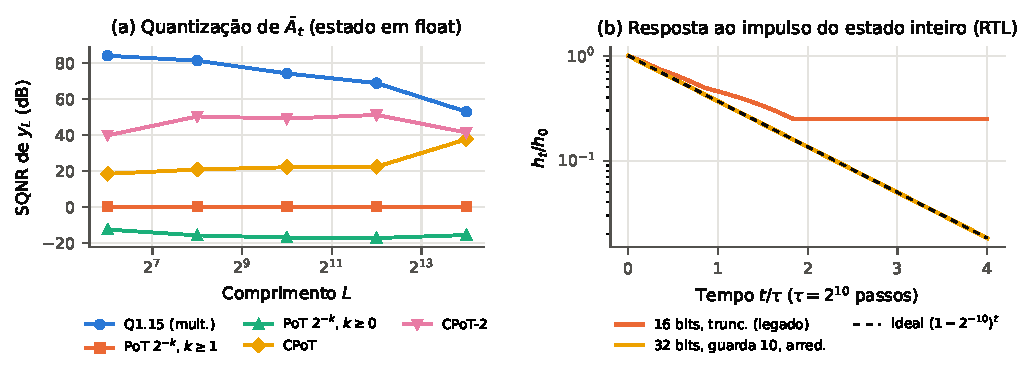
\includegraphics[width=\textwidth]{fig_long_memory.pdf}
  \caption{(a) E2: SQNR da leitura $y_L$ em fun\c{c}\~{a}o de $L$ (estado em float). (b) E3: resposta ao impulso do estado inteiro do RTL com $\bar{A}=1-2^{-10}$. O estado legado de 16 bits congela pouco antes de $2\tau$; o estado corrigido segue a curva ideal.}
  \label{fig:longmem}
\end{figure}

\begin{table}[htb]
\centering
\caption{E3 e E4: estado inteiro do RTL. Raz\~{a}o $h_t/h_t^{\mathrm{ideal}}$ ap\'{o}s $4\tau$ passos de um impulso ($\bar{A} = 1-2^{-k}$) e SQNR do \emph{datapath} inteiro com entradas aleat\'{o}rias (3 sementes).}
\label{tab:state}
\footnotesize
\resizebox{\textwidth}{!}{%
\begin{tabular}{lcccc}
\toprule
\textbf{Estado} & \textbf{$k=8$} & \textbf{$k=10$} & \textbf{$k=12$} & \textbf{SQNR E4 (dB)} \\
\midrule
Legado: 16 bits, sem guarda, truncamento & 3{,}43 & 13{,}66 & 54{,}61 & 37{,}0 \\
Corrigido: 32 bits, 10 bits de guarda, arredondamento & 1{,}00 & 1{,}00 & 1{,}00 & 99{,}0 \\
Baseline: multiplicador Q1.15, 32 bits & --- & --- & --- & 99{,}3 \\
\bottomrule

\end{tabular}}
\end{table}

A Tabela~\ref{tab:state} confirma a an\'{a}lise da Se\c{c}\~{a}o~\ref{sec:precisao}. Com o estado legado (16 bits, truncamento), ap\'{o}s $4\tau$ o estado vale \ImpLegacyTwelve$\times$ o ideal para $k=12$ (e \ImpLegacyEight$\times$ j\'{a} para $k=8$), e o SQNR do \emph{datapath} cai para \SqnrLegacy~dB. Com 32 bits, 10 bits de guarda e arredondamento, a resposta ao impulso coincide com a ideal e o SQNR sobe para \SqnrProposed~dB, no mesmo n\'{\i}vel do baseline com multiplicador (\SqnrMult~dB).

\subsection{Abla\c{c}\~{a}o QAT}

\begin{table}[htb]
\centering
\caption{Acur\'{a}cia de teste (\%, m\'{e}dia $\pm$ desvio padr\~{a}o entre sementes). $^\dagger$/$^\ddagger$: o mesmo modelo treinado, avaliado com o \emph{scan} inteiro bit-exato do RTL.}
\label{tab:ablation}
\footnotesize
\setlength{\tabcolsep}{3pt}
\resizebox{\textwidth}{!}{%
\begin{tabular}{c}\toprule
\textbf{resultados pendentes} \\
\bottomrule
\end{tabular}
}
\end{table}

A Tabela~\ref{tab:ablation} leva a cinco observa\c{c}\~{o}es.

\textbf{ECG5000.} Todas as configura\c{c}\~{o}es ficam a menos de 0,5 ponto percentual da refer\^{e}ncia FP32 (\acc{ecg}{A0}\%), exceto o PoT com $k\geq1$ (\acc{ecg}{A5}\%); o CPoT com \emph{scan} de hardware obt\'{e}m \acc{ecg}{A7}\%. A acur\'{a}cia balanceada fica perto de 52\% em todas as configura\c{c}\~{o}es, inclusive FP32: com 500 s\'{e}ries de treino, as classes minorit\'{a}rias n\~{a}o s\~{a}o aprendidas, o que \'{e} uma limita\c{c}\~{a}o do modelo e do protocolo, n\~{a}o da quantiza\c{c}\~{a}o. Como $L=140$, o estado legado de 16 bits n\~{a}o chega a prejudicar (\acc{ecg}{A7cpots16}\%).

\textbf{Recorda\c{c}\~{a}o com $L=256$.} Todas as configura\c{c}\~{o}es resolvem a tarefa (acur\'{a}cia acima de 90\% em \solved{cueA}{A7} sementes no CPoT), exceto o PoT com $k\geq1$ (\acc{cueA}{A5}\%, n\'{\i}vel de acaso), que n\~{a}o consegue representar $\bar{A}_t > 0{,}5$.

\textbf{Recorda\c{c}\~{a}o com $L=1024$.} FP32, W8A8 e PoT com $k\geq0$ resolvem todas as sementes. Os modelos tern\'{a}rios, \emph{com qualquer} decaimento (A2, A3, A4, A7, A8), resolvem no m\'{a}ximo uma de tr\^{e}s sementes (acur\'{a}cia acima de 90\% em \solved{cueB}{A3} sementes em A3 e em \solved{cueB}{A7} em A7, cuja melhor semente acerta parcialmente); nas demais sementes eles ficam no n\'{\i}vel de acaso. O gargalo nesse comprimento \'{e} a otimiza\c{c}\~{a}o dos pesos tern\'{a}rios dentro do or\c{c}amento usado (20 \'{e}pocas, \TrainCueB{} sequ\^{e}ncias), e n\~{a}o a discretiza\c{c}\~{a}o de $\bar{A}_t$; com 3 sementes, os desvios s\~{a}o grandes e as m\'{e}dias de A2--A8 n\~{a}o permitem ordenar os esquemas.

\textbf{CPoT $\times$ PoT com $k\geq0$.} Nessas tarefas o PoT com $k\geq0$ empata com o CPoT ($L=256$) ou o supera ($L=1024$). A tarefa de recorda\c{c}\~{a}o s\'{o} exige reter informa\c{c}\~{a}o ($\bar{A}_t \to 1$), e o $\Delta_t$ seletivo permite zerar o estado quando necess\'{a}rio; ela n\~{a}o exige constantes de tempo intermedi\'{a}rias, que \'{e} onde o CPoT se diferencia (E1 e E2). Mostrar essa vantagem em acur\'{a}cia exige uma tarefa com esquecimento gradual e ainda est\'{a} em aberto. A FWHT (A2 $\to$ A3) tamb\'{e}m n\~{a}o mostrou efeito mensur\'{a}vel nessas tarefas, que n\~{a}o t\^{e}m canais de \emph{outlier}.

\textbf{Aritm\'{e}tica inteira do RTL.} Avaliar o modelo treinado com o \emph{scan} inteiro bit-exato reproduz a acur\'{a}cia em ponto flutuante (A4$^\dagger$ e A7$^\dagger$, diferen\c{c}as de no m\'{a}ximo alguns d\'{e}cimos). Com o estado legado (A7$^\ddagger$), o mesmo modelo cai de \acc{cueA}{A7cpots32}\% para \acc{cueA}{A7cpots16}\% em $L=256$ e de \acc{cueB}{A7cpots32}\% para \acc{cueB}{A7cpots16}\% em $L=1024$: o problema de precis\~{a}o da Se\c{c}\~{a}o~\ref{sec:precisao} tamb\'{e}m aparece numa tarefa treinada.

Nos modelos tern\'{a}rios treinados, \ZeroFrac{} dos pesos das proje\c{c}\~{o}es valem zero (m\'{e}dia de A7). As proje\c{c}\~{o}es ocupam \ProjKiBfp{}~KiB em FP16, \ProjKiBint{}~KiB em INT8, \ProjKiBtwo{}~KiB em 2 bits e \ProjKiBrthree{}~KiB em Radix-3.

\subsection{Verifica\c{c}\~{a}o do RTL}

\begin{table}[htb]
\centering
\caption{Verifica\c{c}\~{a}o RTL $\times$ modelo de refer\^{e}ncia inteiro (Icarus Verilog 12).}
\label{tab:verif}
\footnotesize
\resizebox{\textwidth}{!}{%
\begin{tabular}{lccc}
\toprule
\textbf{M\'{o}dulo} & \textbf{Configura\c{c}\~{o}es} & \textbf{Sa\'{\i}das comparadas} & \textbf{Diverg\^{e}ncias} \\
\midrule
Decodificador Radix-3 (exaustivo, 256 códigos) & 1 & 256 & 0 \\
FWHT 16 pontos (vetores aleatórios + extremos) & 1 & 2.000 & 0 \\
Motor matriz-vetor (INT8/2-bit/Radix-3, $P\in\{16,32,64\}$) & 9 & 984 & 0 \\
Lane de \emph{scan} (CPoT 32b, CPoT 16b legado, Q1.15) & 3 & 6.144 & 0 \\
\midrule
\textbf{Total} & 14 & \textbf{9.384} & \textbf{0} \\
\bottomrule

\end{tabular}}
\end{table}

Todos os \VerTests{} testes da Tabela~\ref{tab:verif} terminam com zero diverg\^{e}ncias. Nenhum teste foi executado em hardware.

\subsection{Recursos estimados (Yosys, Cyclone~V)}

\begin{table}[htb]
\centering
\caption{Motor matriz-vetor ($K=\EngK$, $M=\EngM$): c\'{e}lulas mapeadas pelo Yosys para Cyclone~V. Ciclos: $MK/P + \log_2 P + 3$, confirmado em simula\c{c}\~{a}o. Sem ALMs/F$_{\max}$ do Quartus.}
\label{tab:engine}
\footnotesize
\resizebox{\textwidth}{!}{%
\begin{tabular}{lcccccccc}
\toprule
\textbf{Pesos} & \textbf{$P$} & \textbf{bit/peso} & \textbf{LUTs} & \textbf{\emph{Carry}} & \textbf{FFs} & \textbf{M10K} & \textbf{Mult. 9$\times$9} & \textbf{Ciclos} \\
\midrule
INT8 (DSP) & 16 & 8{,}00 & 210 & 360 & 844 & 128 & 16 & 8.199 \\
 & 32 & 8{,}00 & 352 & 685 & 1.612 & 128 & 32 & 4.104 \\
 & 64 & 8{,}00 & 893 & 1.338 & 3.148 & 103 & 64 & 2.057 \\
\midrule
Ternário 2-bit & 16 & 2{,}00 & 370 & 304 & 732 & 32 & 0 & 8.199 \\
 & 32 & 2{,}00 & 672 & 573 & 1.388 & 32 & 0 & 4.104 \\
 & 64 & 2{,}00 & 1.533 & 1.114 & 2.700 & 26 & 0 & 2.057 \\
\midrule
Ternário Radix-3 & 16 & 1{,}60 & 1.019 & 305 & 736 & 26 & 0 & 8.199 \\
 & 32 & 1{,}60 & 1.972 & 574 & 1.392 & 26 & 0 & 4.104 \\
 & 64 & 1{,}60 & 4.101 & 1.115 & 2.704 & 26 & 0 & 2.057 \\
\bottomrule

\end{tabular}}
\end{table}

\begin{table}[htb]
\centering
\caption{Blocos do \emph{scan} ($N=16$ estados) e auxiliares: c\'{e}lulas mapeadas pelo Yosys para Cyclone~V e blocos DSP estimados.}
\label{tab:blocks}
\footnotesize
\resizebox{\textwidth}{!}{%
\begin{tabular}{lccccccc}
\toprule
\textbf{Bloco} & \textbf{LUTs} & \textbf{\emph{Carry}} & \textbf{FFs} & \textbf{9$\times$9} & \textbf{18$\times$18} & \textbf{27$\times$27} & \textbf{DSP est.} \\
\midrule
CPoT, 32b + guarda (proposto) & 3.101 & 4.144 & 2.332 & 32 & 0 & 16 & 27 \\
CPoT, 16b (legado, incorreto) & 1.675 & 1.694 & 1.590 & 16 & 16 & 0 & 14 \\
Multiplicador Q1.15, 32b & 2.483 & 3.402 & 2.343 & 64 & 0 & 32 & 54 \\
FWHT 16 pontos & 0 & 720 & 724 & 0 & 0 & 0 & 0 \\
Decodificador Radix-3 (1 byte) & 38 & 0 & 0 & 0 & 0 & 0 & 0 \\
\bottomrule

\end{tabular}}
\end{table}

\textbf{Proje\c{c}\~{o}es (Tabela~\ref{tab:engine}).} Os motores tern\'{a}rios n\~{a}o usam multiplicadores, enquanto o INT8 usa um 9$\times$9 por via (\MulIntA{} com $P=16$). Com $P=16$, a mem\'{o}ria de pesos cai de \MtenkIntA{} blocos M10K (INT8) para \MtenkTwoA{} (2-bit) e \MtenkRthreeA{} (Radix-3). O Radix-3 custa LUTs: \LutRthreeA{} contra \LutTwoA{} no 2-bit com $P=16$, porque cada via tem um decodificador (\LutDec{} LUTs) e um multiplexador 5:1. Com $P=64$ a vantagem em M10K desaparece (\MtenkTwoC{} contra \MtenkRthreeC{} blocos): a largura da palavra, e n\~{a}o o total de bits, define o n\'{u}mero de blocos, enquanto o custo em LUTs sobe para \LutRthreeC{} contra \LutTwoC. A economia de 20\% em bits do Radix-3 s\'{o} se traduz em blocos quando a geometria da mem\'{o}ria permite, ou em banda quando os pesos v\^{e}m da DRAM, regime que n\~{a}o foi medido.

\textbf{\emph{Scan} (Tabela~\ref{tab:blocks}).} O decaimento CPoT elimina os multiplicadores $h \cdot \bar{A}$: a \emph{lane} proposta usa \DspCpot{} blocos DSP estimados contra \DspMult{} do baseline Q1.15, ao custo de mais l\'{o}gica (\LutCpot{} contra \LutMult{} LUTs, devido ao deslocador de 32 bits). Os DSPs restantes v\^{e}m de $B_t x_t$ e $C_t h_t$, que continuam sendo multiplica\c{c}\~{o}es. A Cyclone~V \texttt{5CSEBA6U23I7} tem 112 blocos DSP, ent\~{a}o o n\'{u}mero de \emph{lanes} paralelas \'{e} limitado por DSP no baseline e por esses produtos no CPoT.

% =============================================================================
\section{Limita\c{c}\~{o}es e Pr\'{o}ximos Passos}
\label{sec:limitacoes}
% =============================================================================

\begin{itemize}
  \item \textbf{Sem Quartus e sem placa.} Os recursos s\~{a}o c\'{e}lulas do Yosys, n\~{a}o ALMs do \emph{fitter}, e n\~{a}o h\'{a} F$_{\max}$, \emph{throughput}, lat\^{e}ncia nem pot\^{e}ncia. A pr\'{o}xima etapa \'{e} rodar \path{synth_quartus.py} e medir na DE10-Nano (ARM via ponte AXI, contadores de ciclo, medidor de corrente na alimenta\c{c}\~{a}o).
  \item \textbf{Integra\c{c}\~{a}o incompleta.} RMSNorm, quantiza\c{c}\~{a}o din\^{a}mica, \texttt{Conv1D}, SiLU e o controle do bloco n\~{a}o est\~{a}o em RTL. No QAT, a FWHT recebe a ativa\c{c}\~{a}o em ponto flutuante; no hardware, ela receber\'{a} INT8 j\'{a} quantizado.
  \item \textbf{Escala.} Modelos pequenos ($\approx$\NParams{} par\^{a}metros) e tarefas de classifica\c{c}\~{a}o; a tarefa de recorda\c{c}\~{a}o \'{e} sint\'{e}tica. Modelos de linguagem e o regime com pesos na DRAM (\emph{memory-bound}) n\~{a}o foram avaliados.
  \item \textbf{Alternativas de motor.} Multiplica\c{c}\~{a}o por tabela (TLMM) e salto de pesos nulos n\~{a}o foram implementados nesta vers\~{a}o.
\end{itemize}

% =============================================================================
\section{Conclus\~{a}o}
% =============================================================================

Apresentamos o BitMamba-CV, um co-projeto de Mamba-2 tern\'{a}rio e de um \emph{datapath} de \emph{scan} para a Intel Cyclone~V, com especifica\c{c}\~{a}o inteira \'{u}nica, RTL verificado bit a bit (\VerTotal{} sa\'{\i}das, \VerMism{} diverg\^{e}ncias) e todos os n\'{u}meros gerados a partir dos resultados. Tr\^{e}s conclus\~{o}es se sustentam com os dados atuais. (i) A discretiza\c{c}\~{a}o CPoT representa constantes de tempo longas com um deslocamento e uma subtra\c{c}\~{a}o (erro mediano de $\tau$ de \TauErrCpot{} em $[0{,}90;\,0{,}999]$, contra \TauErrPot{} do PoT com $k\geq1$) e reduz os blocos DSP estimados da \emph{lane} de \emph{scan} de \DspMult{} para \DspCpot. (ii) Essa discretiza\c{c}\~{a}o s\'{o} \'{e} correta com estado de 32 bits, bits de guarda e arredondamento: o estado de 16 bits truncado congela a mem\'{o}ria longa, derruba o SQNR do \emph{datapath} de \SqnrProposed{} para \SqnrLegacy~dB e a acur\'{a}cia da tarefa de recorda\c{c}\~{a}o com $L=256$ de \acc{cueA}{A7cpots32}\% para \acc{cueA}{A7cpots16}\%. (iii) O modelo tern\'{a}rio com \emph{scan} inteiro mant\'{e}m a acur\'{a}cia FP32 no ECG5000 e na recorda\c{c}\~{a}o com $L=256$; com $L=1024$, o treinamento tern\'{a}rio n\~{a}o converge na maioria das sementes. Ficam em aberto: a vantagem do CPoT sobre o PoT com $k\geq0$ em acur\'{a}cia, a s\'{\i}ntese no Quartus (ALMs e F$_{\max}$) e a valida\c{c}\~{a}o na placa DE10-Nano (lat\^{e}ncia e pot\^{e}ncia).

\bibliographystyle{plain}
\bibliography{references}

\end{document}
